\documentclass[1p]{elsarticle_modified}
%\bibliographystyle{elsarticle-num}

%\usepackage[colorlinks]{hyperref}
%\usepackage{abbrmath_seonhwa} %\Abb, \Ascr, \Acal ,\Abf, \Afrak
\usepackage{amsfonts}
\usepackage{amssymb}
\usepackage{amsmath}
\usepackage{amsthm}
\usepackage{scalefnt}
\usepackage{amsbsy}
\usepackage{kotex}
\usepackage{caption}
\usepackage{subfig}
\usepackage{color}
\usepackage{graphicx}
\usepackage{xcolor} %% white, black, red, green, blue, cyan, magenta, yellow
\usepackage{float}
\usepackage{setspace}
\usepackage{hyperref}

\usepackage{tikz}
\usetikzlibrary{arrows}

\usepackage{multirow}
\usepackage{array} % fixed length table
\usepackage{hhline}

%%%%%%%%%%%%%%%%%%%%%
\makeatletter
\renewcommand*\env@matrix[1][\arraystretch]{%
	\edef\arraystretch{#1}%
	\hskip -\arraycolsep
	\let\@ifnextchar\new@ifnextchar
	\array{*\c@MaxMatrixCols c}}
\makeatother %https://tex.stackexchange.com/questions/14071/how-can-i-increase-the-line-spacing-in-a-matrix
%%%%%%%%%%%%%%%

\usepackage[normalem]{ulem}

\newcommand{\msout}[1]{\ifmmode\text{\sout{\ensuremath{#1}}}\else\sout{#1}\fi}
%SOURCE: \msout is \stkout macro in https://tex.stackexchange.com/questions/20609/strikeout-in-math-mode

\newcommand{\cancel}[1]{
	\ifmmode
	{\color{red}\msout{#1}}
	\else
	{\color{red}\sout{#1}}
	\fi
}

\newcommand{\add}[1]{
	{\color{blue}\uwave{#1}}
}

\newcommand{\replace}[2]{
	\ifmmode
	{\color{red}\msout{#1}}{\color{blue}\uwave{#2}}
	\else
	{\color{red}\sout{#1}}{\color{blue}\uwave{#2}}
	\fi
}

\newcommand{\Sol}{\mathcal{S}} %segment
\newcommand{\D}{D} %diagram
\newcommand{\A}{\mathcal{A}} %arc


%%%%%%%%%%%%%%%%%%%%%%%%%%%%%5 test

\def\sl{\operatorname{\textup{SL}}(2,\Cbb)}
\def\psl{\operatorname{\textup{PSL}}(2,\Cbb)}
\def\quan{\mkern 1mu \triangleright \mkern 1mu}

\theoremstyle{definition}
\newtheorem{thm}{Theorem}[section]
\newtheorem{prop}[thm]{Proposition}
\newtheorem{lem}[thm]{Lemma}
\newtheorem{ques}[thm]{Question}
\newtheorem{cor}[thm]{Corollary}
\newtheorem{defn}[thm]{Definition}
\newtheorem{exam}[thm]{Example}
\newtheorem{rmk}[thm]{Remark}
\newtheorem{alg}[thm]{Algorithm}

\newcommand{\I}{\sqrt{-1}}
\begin{document}

%\begin{frontmatter}
%
%\title{Boundary parabolic representations of knots up to 8 crossings}
%
%%% Group authors per affiliation:
%\author{Yunhi Cho} 
%\address{Department of Mathematics, University of Seoul, Seoul, Korea}
%\ead{yhcho@uos.ac.kr}
%
%
%\author{Seonhwa Kim} %\fnref{s_kim}}
%\address{Center for Geometry and Physics, Institute for Basic Science, Pohang, 37673, Korea}
%\ead{ryeona17@ibs.re.kr}
%
%\author{Hyuk Kim}
%\address{Department of Mathematical Sciences, Seoul National University, Seoul 08826, Korea}
%\ead{hyukkim@snu.ac.kr}
%
%\author{Seokbeom Yoon}
%\address{Department of Mathematical Sciences, Seoul National University, Seoul, 08826,  Korea}
%\ead{sbyoon15@snu.ac.kr}
%
%\begin{abstract}
%We find all boundary parabolic representation of knots up to 8 crossings.
%
%\end{abstract}
%\begin{keyword}
%    \MSC[2010] 57M25 
%\end{keyword}
%
%\end{frontmatter}

%\linenumbers
%\tableofcontents
%
\newcommand\colored[1]{\textcolor{white}{\rule[-0.35ex]{0.8em}{1.4ex}}\kern-0.8em\color{red} #1}%
%\newcommand\colored[1]{\textcolor{white}{ #1}\kern-2.17ex	\textcolor{white}{ #1}\kern-1.81ex	\textcolor{white}{ #1}\kern-2.15ex\color{red}#1	}

{\Large $\underline{10_{110}~(K10a_{100})}$}

\setlength{\tabcolsep}{10pt}
\renewcommand{\arraystretch}{1.6}
\vspace{1cm}\begin{tabular}{m{100pt}>{\centering\arraybackslash}m{274pt}}
\multirow{5}{120pt}{
	\centering
	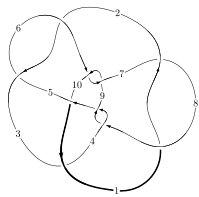
\includegraphics[width=112pt]{../../../GIT/diagram.site/Diagrams/png/194_10_110.png}\\
\ \ \ A knot diagram\footnotemark}&
\allowdisplaybreaks
\textbf{Linearized knot diagam} \\
\cline{2-2}
 &
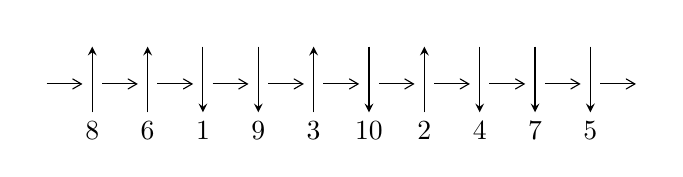
\begin{tikzpicture}[x=20pt, y=17pt]
	% nodes
	\node (C0) at (0, 0) {};
	\node (C1) at (1, 0) {};
	\node (C1U) at (1, +1) {};
	\node (C1D) at (1, -1) {8};

	\node (C2) at (2, 0) {};
	\node (C2U) at (2, +1) {};
	\node (C2D) at (2, -1) {6};

	\node (C3) at (3, 0) {};
	\node (C3U) at (3, +1) {};
	\node (C3D) at (3, -1) {1};

	\node (C4) at (4, 0) {};
	\node (C4U) at (4, +1) {};
	\node (C4D) at (4, -1) {9};

	\node (C5) at (5, 0) {};
	\node (C5U) at (5, +1) {};
	\node (C5D) at (5, -1) {3};

	\node (C6) at (6, 0) {};
	\node (C6U) at (6, +1) {};
	\node (C6D) at (6, -1) {10};

	\node (C7) at (7, 0) {};
	\node (C7U) at (7, +1) {};
	\node (C7D) at (7, -1) {2};

	\node (C8) at (8, 0) {};
	\node (C8U) at (8, +1) {};
	\node (C8D) at (8, -1) {4};

	\node (C9) at (9, 0) {};
	\node (C9U) at (9, +1) {};
	\node (C9D) at (9, -1) {7};

	\node (C10) at (10, 0) {};
	\node (C10U) at (10, +1) {};
	\node (C10D) at (10, -1) {5};
	\node (C11) at (11, 0) {};

	% arrows
	\draw[->,>={angle 60}]
	(C0) edge (C1) (C1) edge (C2) (C2) edge (C3) (C3) edge (C4) (C4) edge (C5) (C5) edge (C6) (C6) edge (C7) (C7) edge (C8) (C8) edge (C9) (C9) edge (C10) (C10) edge (C11) ;	\draw[->,>=stealth]
	(C1D) edge (C1U) (C2D) edge (C2U) (C3U) edge (C3D) (C4U) edge (C4D) (C5D) edge (C5U) (C6U) edge (C6D) (C7D) edge (C7U) (C8U) edge (C8D) (C9U) edge (C9D) (C10U) edge (C10D) ;
	\end{tikzpicture} \\
\hhline{~~} \\& 
\textbf{Solving Sequence} \\ \cline{2-2} 
 &
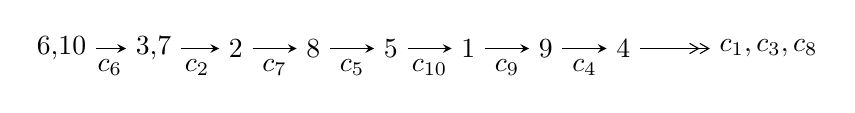
\begin{tikzpicture}[x=28pt, y=7pt]
	% node
	\node (A0) at (-1/8, 0) {6,10};
	\node (A1) at (17/16, 0) {3,7};
	\node (A2) at (17/8, 0) {2};
	\node (A3) at (25/8, 0) {8};
	\node (A4) at (33/8, 0) {5};
	\node (A5) at (41/8, 0) {1};
	\node (A6) at (49/8, 0) {9};
	\node (A7) at (57/8, 0) {4};
	\node (C1) at (1/2, -1) {$c_{6}$};
	\node (C2) at (13/8, -1) {$c_{2}$};
	\node (C3) at (21/8, -1) {$c_{7}$};
	\node (C4) at (29/8, -1) {$c_{5}$};
	\node (C5) at (37/8, -1) {$c_{10}$};
	\node (C6) at (45/8, -1) {$c_{9}$};
	\node (C7) at (53/8, -1) {$c_{4}$};
	\node (A8) at (9, 0) {$c_{1},c_{3},c_{8}$};

	% edge
	\draw[->,>=stealth]	
	(A0) edge (A1) (A1) edge (A2) (A2) edge (A3) (A3) edge (A4) (A4) edge (A5) (A5) edge (A6) (A6) edge (A7) ;
	\draw[->>,>={angle 60}]	
	(A7) edge (A8);
\end{tikzpicture} \\ 

\end{tabular} \\

\footnotetext{
The image of knot diagram is generated by the software ``\textbf{Draw programme}" developed by Andrew Bartholomew(\url{http://www.layer8.co.uk/maths/draw/index.htm\#Running-draw}), where we modified some parts for our purpose(\url{https://github.com/CATsTAILs/LinksPainter}).
}\phantom \\ \newline 
\centering \textbf{Ideals for irreducible components\footnotemark of $X_{\text{par}}$} 
 
\begin{align*}
I^u_{1}&=\langle 
-3.94814\times10^{60} u^{50}+1.33577\times10^{61} u^{49}+\cdots+7.13614\times10^{60} b+1.16812\times10^{61},\\
\phantom{I^u_{1}}&\phantom{= \langle  }4.97115\times10^{60} u^{50}-4.93286\times10^{59} u^{49}+\cdots+7.13614\times10^{60} a+1.37929\times10^{62},\;u^{51}-3 u^{50}+\cdots-3 u+1\rangle \\
I^u_{2}&=\langle 
- u^9+3 u^8-8 u^7+11 u^6-14 u^5+10 u^4-9 u^3+5 u^2+b-4 u+1,\\
\phantom{I^u_{2}}&\phantom{= \langle  }-2 u^9+4 u^8-12 u^7+12 u^6-20 u^5+10 u^4-17 u^3+3 u^2+a-7 u-1,\\
\phantom{I^u_{2}}&\phantom{= \langle  }u^{10}-2 u^9+6 u^8-6 u^7+10 u^6-5 u^5+9 u^4-2 u^3+5 u^2+1\rangle \\
\\
\end{align*}
\raggedright * 2 irreducible components of $\dim_{\mathbb{C}}=0$, with total 61 representations.\\
\footnotetext{All coefficients of polynomials are rational numbers. But the coefficients are sometimes approximated in decimal forms when there is not enough margin.}
\newpage
\renewcommand{\arraystretch}{1}
\centering \section*{I. $I^u_{1}= \langle -3.95\times10^{60} u^{50}+1.34\times10^{61} u^{49}+\cdots+7.14\times10^{60} b+1.17\times10^{61},\;4.97\times10^{60} u^{50}-4.93\times10^{59} u^{49}+\cdots+7.14\times10^{60} a+1.38\times10^{62},\;u^{51}-3 u^{50}+\cdots-3 u+1 \rangle$}
\flushleft \textbf{(i) Arc colorings}\\
\begin{tabular}{m{7pt} m{180pt} m{7pt} m{180pt} }
\flushright $a_{6}=$&$\begin{pmatrix}1\\0\end{pmatrix}$ \\
\flushright $a_{10}=$&$\begin{pmatrix}0\\u\end{pmatrix}$ \\
\flushright $a_{3}=$&$\begin{pmatrix}-0.696616 u^{50}+0.0691250 u^{49}+\cdots+26.3979 u-19.3282\\0.553261 u^{50}-1.87184 u^{49}+\cdots+6.93494 u-1.63690\end{pmatrix}$ \\
\flushright $a_{7}=$&$\begin{pmatrix}1\\u^2\end{pmatrix}$ \\
\flushright $a_{2}=$&$\begin{pmatrix}-1.24988 u^{50}+1.94096 u^{49}+\cdots+19.4629 u-17.6913\\0.553261 u^{50}-1.87184 u^{49}+\cdots+6.93494 u-1.63690\end{pmatrix}$ \\
\flushright $a_{8}=$&$\begin{pmatrix}5.62576 u^{50}-16.6964 u^{49}+\cdots+84.9147 u-14.4475\\1.31452 u^{50}-3.25740 u^{49}+\cdots+7.88805 u+0.493476\end{pmatrix}$ \\
\flushright $a_{5}=$&$\begin{pmatrix}-5.07269 u^{50}+14.7750 u^{49}+\cdots-63.8914 u+8.27803\\-0.685403 u^{50}+1.65384 u^{49}+\cdots-3.62278 u-0.452805\end{pmatrix}$ \\
\flushright $a_{1}=$&$\begin{pmatrix}2.36727 u^{50}-7.12893 u^{49}+\cdots+76.0899 u-9.67668\\-1.36131 u^{50}+4.21987 u^{49}+\cdots-3.74774 u+3.48147\end{pmatrix}$ \\
\flushright $a_{9}=$&$\begin{pmatrix}u\\u^3+u\end{pmatrix}$ \\
\flushright $a_{4}=$&$\begin{pmatrix}-5.82333 u^{50}+16.7794 u^{49}+\cdots-68.9333 u+8.68998\\-1.34927 u^{50}+3.56133 u^{49}+\cdots-8.65673 u+0.206715\end{pmatrix}$\\&\end{tabular}
\flushleft \textbf{(ii) Obstruction class $= -1$}\\~\\
\flushleft \textbf{(iii) Cusp Shapes $= 0.603997 u^{50}-6.94205 u^{49}+\cdots+39.9158 u-23.3331$}\\~\\
\newpage\renewcommand{\arraystretch}{1}
\flushleft \textbf{(iv) u-Polynomials at the component}\newline \\
\begin{tabular}{m{50pt}|m{274pt}}
Crossings & \hspace{64pt}u-Polynomials at each crossing \\
\hline $$\begin{aligned}c_{1},c_{7}\end{aligned}$$&$\begin{aligned}
&u^{51}- u^{50}+\cdots+559 u+143
\end{aligned}$\\
\hline $$\begin{aligned}c_{2},c_{5}\end{aligned}$$&$\begin{aligned}
&u^{51}+3 u^{50}+\cdots+97 u+17
\end{aligned}$\\
\hline $$\begin{aligned}c_{3}\end{aligned}$$&$\begin{aligned}
&u^{51}-3 u^{50}+\cdots+2441 u-1003
\end{aligned}$\\
\hline $$\begin{aligned}c_{4},c_{8}\end{aligned}$$&$\begin{aligned}
&u^{51}- u^{50}+\cdots+20 u+23
\end{aligned}$\\
\hline $$\begin{aligned}c_{6},c_{9}\end{aligned}$$&$\begin{aligned}
&u^{51}-3 u^{50}+\cdots-3 u+1
\end{aligned}$\\
\hline $$\begin{aligned}c_{10}\end{aligned}$$&$\begin{aligned}
&u^{51}+u^{50}+\cdots+118 u+47
\end{aligned}$\\
\hline
\end{tabular}\\~\\
\newpage\renewcommand{\arraystretch}{1}
\flushleft \textbf{(v) Riley Polynomials at the component}\newline \\
\begin{tabular}{m{50pt}|m{274pt}}
Crossings & \hspace{64pt}Riley Polynomials at each crossing \\
\hline $$\begin{aligned}c_{1},c_{7}\end{aligned}$$&$\begin{aligned}
&y^{51}+41 y^{50}+\cdots-137683 y-20449
\end{aligned}$\\
\hline $$\begin{aligned}c_{2},c_{5}\end{aligned}$$&$\begin{aligned}
&y^{51}+33 y^{50}+\cdots-4701 y-289
\end{aligned}$\\
\hline $$\begin{aligned}c_{3}\end{aligned}$$&$\begin{aligned}
&y^{51}-23 y^{50}+\cdots+17745737 y-1006009
\end{aligned}$\\
\hline $$\begin{aligned}c_{4},c_{8}\end{aligned}$$&$\begin{aligned}
&y^{51}-35 y^{50}+\cdots+3022 y-529
\end{aligned}$\\
\hline $$\begin{aligned}c_{6},c_{9}\end{aligned}$$&$\begin{aligned}
&y^{51}+27 y^{50}+\cdots-45 y-1
\end{aligned}$\\
\hline $$\begin{aligned}c_{10}\end{aligned}$$&$\begin{aligned}
&y^{51}-9 y^{50}+\cdots+9976 y-2209
\end{aligned}$\\
\hline
\end{tabular}\\~\\
\newpage\flushleft \textbf{(vi) Complex Volumes and Cusp Shapes}
$$\begin{array}{c|c|c}  
\text{Solutions to }I^u_{1}& \I (\text{vol} + \sqrt{-1}CS) & \text{Cusp shape}\\
 \hline 
\begin{aligned}
u &= -0.994943 + 0.185745 I \\
a &= \phantom{-}0.422541 - 1.311700 I \\
b &= \phantom{-}0.266229 - 1.334950 I\end{aligned}
 & -5.72149 - 2.82797 I & -6.95847 + 2.49384 I \\ \hline\begin{aligned}
u &= -0.994943 - 0.185745 I \\
a &= \phantom{-}0.422541 + 1.311700 I \\
b &= \phantom{-}0.266229 + 1.334950 I\end{aligned}
 & -5.72149 + 2.82797 I & -6.95847 - 2.49384 I \\ \hline\begin{aligned}
u &= \phantom{-}0.390188 + 0.947913 I \\
a &= -1.03830 - 1.40939 I \\
b &= \phantom{-}0.516208 - 1.186450 I\end{aligned}
 & \phantom{-}0.72717 - 4.12473 I & \phantom{-}0.68433 + 2.44113 I \\ \hline\begin{aligned}
u &= \phantom{-}0.390188 - 0.947913 I \\
a &= -1.03830 + 1.40939 I \\
b &= \phantom{-}0.516208 + 1.186450 I\end{aligned}
 & \phantom{-}0.72717 + 4.12473 I & \phantom{-}0.68433 - 2.44113 I \\ \hline\begin{aligned}
u &= -0.375762 + 0.890024 I \\
a &= -0.426976 + 0.241699 I \\
b &= \phantom{-}1.350530 - 0.349643 I\end{aligned}
 & \phantom{-}0.99311 + 1.57122 I & -7.65217 - 5.55090 I \\ \hline\begin{aligned}
u &= -0.375762 - 0.890024 I \\
a &= -0.426976 - 0.241699 I \\
b &= \phantom{-}1.350530 + 0.349643 I\end{aligned}
 & \phantom{-}0.99311 - 1.57122 I & -7.65217 + 5.55090 I \\ \hline\begin{aligned}
u &= \phantom{-}0.019775 + 1.071160 I \\
a &= -0.261242 - 0.274009 I \\
b &= \phantom{-}0.863662 + 0.336843 I\end{aligned}
 & \phantom{-}3.46242 + 0.95472 I & \phantom{-}4.42129 - 1.75327 I \\ \hline\begin{aligned}
u &= \phantom{-}0.019775 - 1.071160 I \\
a &= -0.261242 + 0.274009 I \\
b &= \phantom{-}0.863662 - 0.336843 I\end{aligned}
 & \phantom{-}3.46242 - 0.95472 I & \phantom{-}4.42129 + 1.75327 I \\ \hline\begin{aligned}
u &= \phantom{-}0.420839 + 1.017200 I \\
a &= -1.97618 - 0.11378 I \\
b &= \phantom{-}0.108632 - 1.103460 I\end{aligned}
 & -6.80830 - 3.96373 I & -9.29905 + 4.39229 I \\ \hline\begin{aligned}
u &= \phantom{-}0.420839 - 1.017200 I \\
a &= -1.97618 + 0.11378 I \\
b &= \phantom{-}0.108632 + 1.103460 I\end{aligned}
 & -6.80830 + 3.96373 I & -9.29905 - 4.39229 I\\
 \hline 
 \end{array}$$\newpage$$\begin{array}{c|c|c}  
\text{Solutions to }I^u_{1}& \I (\text{vol} + \sqrt{-1}CS) & \text{Cusp shape}\\
 \hline 
\begin{aligned}
u &= \phantom{-}0.526532 + 0.993852 I \\
a &= \phantom{-}1.216580 + 0.601262 I \\
b &= -0.68843 + 1.24828 I\end{aligned}
 & -7.65143 - 1.97817 I & -7.82727 + 2.61940 I \\ \hline\begin{aligned}
u &= \phantom{-}0.526532 - 0.993852 I \\
a &= \phantom{-}1.216580 - 0.601262 I \\
b &= -0.68843 - 1.24828 I\end{aligned}
 & -7.65143 + 1.97817 I & -7.82727 - 2.61940 I \\ \hline\begin{aligned}
u &= \phantom{-}0.506288 + 0.633852 I \\
a &= -0.296136 - 0.899365 I \\
b &= -0.37733 - 1.57824 I\end{aligned}
 & -8.80240 - 2.26810 I & -9.50846 + 5.46846 I \\ \hline\begin{aligned}
u &= \phantom{-}0.506288 - 0.633852 I \\
a &= -0.296136 + 0.899365 I \\
b &= -0.37733 + 1.57824 I\end{aligned}
 & -8.80240 + 2.26810 I & -9.50846 - 5.46846 I \\ \hline\begin{aligned}
u &= \phantom{-}0.557126 + 1.094830 I \\
a &= \phantom{-}0.113684 + 0.264643 I \\
b &= -1.213990 - 0.101030 I\end{aligned}
 & -3.13564 - 8.43581 I & \phantom{-0.000000 } 0 \\ \hline\begin{aligned}
u &= \phantom{-}0.557126 - 1.094830 I \\
a &= \phantom{-}0.113684 - 0.264643 I \\
b &= -1.213990 + 0.101030 I\end{aligned}
 & -3.13564 + 8.43581 I & \phantom{-0.000000 } 0 \\ \hline\begin{aligned}
u &= -0.113572 + 1.239660 I \\
a &= \phantom{-}0.242019 + 0.693111 I \\
b &= -0.450396 + 0.753572 I\end{aligned}
 & -0.289715 + 0.727443 I & \phantom{-0.000000 } 0 \\ \hline\begin{aligned}
u &= -0.113572 - 1.239660 I \\
a &= \phantom{-}0.242019 - 0.693111 I \\
b &= -0.450396 - 0.753572 I\end{aligned}
 & -0.289715 - 0.727443 I & \phantom{-0.000000 } 0 \\ \hline\begin{aligned}
u &= -0.520426 + 1.134500 I \\
a &= \phantom{-}1.06013 - 1.60375 I \\
b &= -0.390004 - 1.272450 I\end{aligned}
 & -2.08580 + 7.78838 I & \phantom{-0.000000 } 0 \\ \hline\begin{aligned}
u &= -0.520426 - 1.134500 I \\
a &= \phantom{-}1.06013 + 1.60375 I \\
b &= -0.390004 + 1.272450 I\end{aligned}
 & -2.08580 - 7.78838 I & \phantom{-0.000000 } 0\\
 \hline 
 \end{array}$$\newpage$$\begin{array}{c|c|c}  
\text{Solutions to }I^u_{1}& \I (\text{vol} + \sqrt{-1}CS) & \text{Cusp shape}\\
 \hline 
\begin{aligned}
u &= \phantom{-}0.332771 + 0.672789 I \\
a &= -0.20644 + 2.43715 I \\
b &= \phantom{-}0.02668 + 1.44197 I\end{aligned}
 & -8.06580 + 0.63479 I & -8.35698 + 2.72496 I \\ \hline\begin{aligned}
u &= \phantom{-}0.332771 - 0.672789 I \\
a &= -0.20644 - 2.43715 I \\
b &= \phantom{-}0.02668 - 1.44197 I\end{aligned}
 & -8.06580 - 0.63479 I & -8.35698 - 2.72496 I \\ \hline\begin{aligned}
u &= -0.314342 + 1.210610 I \\
a &= \phantom{-}0.219903 - 0.392050 I \\
b &= -0.672500 + 0.034322 I\end{aligned}
 & \phantom{-}1.72349 + 3.73342 I & \phantom{-0.000000 } 0 \\ \hline\begin{aligned}
u &= -0.314342 - 1.210610 I \\
a &= \phantom{-}0.219903 + 0.392050 I \\
b &= -0.672500 - 0.034322 I\end{aligned}
 & \phantom{-}1.72349 - 3.73342 I & \phantom{-0.000000 } 0 \\ \hline\begin{aligned}
u &= -0.741826 + 1.022810 I \\
a &= -0.261173 + 1.316850 I \\
b &= \phantom{-}0.149560 + 1.061710 I\end{aligned}
 & -1.24787 + 2.87055 I & \phantom{-0.000000 } 0 \\ \hline\begin{aligned}
u &= -0.741826 - 1.022810 I \\
a &= -0.261173 - 1.316850 I \\
b &= \phantom{-}0.149560 - 1.061710 I\end{aligned}
 & -1.24787 - 2.87055 I & \phantom{-0.000000 } 0 \\ \hline\begin{aligned}
u &= -0.724864\phantom{ +0.000000I} \\
a &= -0.327919\phantom{ +0.000000I} \\
b &= -0.557789\phantom{ +0.000000I}\end{aligned}
 & -2.02066\phantom{ +0.000000I} & -3.93810\phantom{ +0.000000I} \\ \hline\begin{aligned}
u &= \phantom{-}0.098596 + 0.711899 I \\
a &= \phantom{-}1.069920 + 0.850725 I \\
b &= -0.054343 + 0.710997 I\end{aligned}
 & -0.177529 + 1.103040 I & -2.91668 - 3.58562 I \\ \hline\begin{aligned}
u &= \phantom{-}0.098596 - 0.711899 I \\
a &= \phantom{-}1.069920 - 0.850725 I \\
b &= -0.054343 - 0.710997 I\end{aligned}
 & -0.177529 - 1.103040 I & -2.91668 + 3.58562 I \\ \hline\begin{aligned}
u &= \phantom{-}0.657571 + 1.111660 I \\
a &= \phantom{-}0.137365 + 0.376163 I \\
b &= \phantom{-}0.663637 + 0.521850 I\end{aligned}
 & -1.42681 - 1.13458 I & \phantom{-0.000000 } 0\\
 \hline 
 \end{array}$$\newpage$$\begin{array}{c|c|c}  
\text{Solutions to }I^u_{1}& \I (\text{vol} + \sqrt{-1}CS) & \text{Cusp shape}\\
 \hline 
\begin{aligned}
u &= \phantom{-}0.657571 - 1.111660 I \\
a &= \phantom{-}0.137365 - 0.376163 I \\
b &= \phantom{-}0.663637 - 0.521850 I\end{aligned}
 & -1.42681 + 1.13458 I & \phantom{-0.000000 } 0 \\ \hline\begin{aligned}
u &= \phantom{-}0.610559 + 0.310111 I \\
a &= \phantom{-}0.21593 + 1.41416 I \\
b &= -0.723237 - 0.300626 I\end{aligned}
 & -5.30063 + 3.74184 I & -6.50172 - 2.38693 I \\ \hline\begin{aligned}
u &= \phantom{-}0.610559 - 0.310111 I \\
a &= \phantom{-}0.21593 - 1.41416 I \\
b &= -0.723237 + 0.300626 I\end{aligned}
 & -5.30063 - 3.74184 I & -6.50172 + 2.38693 I \\ \hline\begin{aligned}
u &= -0.681382 + 0.037993 I \\
a &= \phantom{-}0.18190 + 2.70537 I \\
b &= -0.349930 + 1.034050 I\end{aligned}
 & -4.86621 - 3.30300 I & -8.47560 + 3.00422 I \\ \hline\begin{aligned}
u &= -0.681382 - 0.037993 I \\
a &= \phantom{-}0.18190 - 2.70537 I \\
b &= -0.349930 - 1.034050 I\end{aligned}
 & -4.86621 + 3.30300 I & -8.47560 - 3.00422 I \\ \hline\begin{aligned}
u &= -0.611419 + 1.218010 I \\
a &= -0.827531 + 0.976005 I \\
b &= \phantom{-}0.63737 + 1.37202 I\end{aligned}
 & -2.65938 + 8.52301 I & \phantom{-0.000000 } 0 \\ \hline\begin{aligned}
u &= -0.611419 - 1.218010 I \\
a &= -0.827531 - 0.976005 I \\
b &= \phantom{-}0.63737 - 1.37202 I\end{aligned}
 & -2.65938 - 8.52301 I & \phantom{-0.000000 } 0 \\ \hline\begin{aligned}
u &= \phantom{-}1.283370 + 0.473849 I \\
a &= -0.337325 - 1.255760 I \\
b &= -0.381442 - 1.278540 I\end{aligned}
 & -9.75856 + 7.66724 I & \phantom{-0.000000 } 0 \\ \hline\begin{aligned}
u &= \phantom{-}1.283370 - 0.473849 I \\
a &= -0.337325 + 1.255760 I \\
b &= -0.381442 + 1.278540 I\end{aligned}
 & -9.75856 - 7.66724 I & \phantom{-0.000000 } 0 \\ \hline\begin{aligned}
u &= -0.732019 + 1.169240 I \\
a &= \phantom{-}0.788213 - 0.967707 I \\
b &= -0.299489 - 0.952219 I\end{aligned}
 & -0.86031 + 3.69765 I & \phantom{-0.000000 } 0\\
 \hline 
 \end{array}$$\newpage$$\begin{array}{c|c|c}  
\text{Solutions to }I^u_{1}& \I (\text{vol} + \sqrt{-1}CS) & \text{Cusp shape}\\
 \hline 
\begin{aligned}
u &= -0.732019 - 1.169240 I \\
a &= \phantom{-}0.788213 + 0.967707 I \\
b &= -0.299489 + 0.952219 I\end{aligned}
 & -0.86031 - 3.69765 I & \phantom{-0.000000 } 0 \\ \hline\begin{aligned}
u &= \phantom{-}1.03951 + 0.98801 I \\
a &= -0.44530 - 1.37365 I \\
b &= \phantom{-}0.511570 - 0.950776 I\end{aligned}
 & -2.64694 - 5.68594 I & \phantom{-0.000000 } 0 \\ \hline\begin{aligned}
u &= \phantom{-}1.03951 - 0.98801 I \\
a &= -0.44530 + 1.37365 I \\
b &= \phantom{-}0.511570 + 0.950776 I\end{aligned}
 & -2.64694 + 5.68594 I & \phantom{-0.000000 } 0 \\ \hline\begin{aligned}
u &= \phantom{-}0.75895 + 1.26498 I \\
a &= \phantom{-}0.81447 + 1.23333 I \\
b &= -0.60063 + 1.36529 I\end{aligned}
 & -7.1442 - 14.7775 I & \phantom{-0.000000 } 0 \\ \hline\begin{aligned}
u &= \phantom{-}0.75895 - 1.26498 I \\
a &= \phantom{-}0.81447 - 1.23333 I \\
b &= -0.60063 - 1.36529 I\end{aligned}
 & -7.1442 + 14.7775 I & \phantom{-0.000000 } 0 \\ \hline\begin{aligned}
u &= \phantom{-}0.004627 + 0.461649 I \\
a &= \phantom{-}1.30111 + 0.61627 I \\
b &= \phantom{-}0.111178 + 0.551129 I\end{aligned}
 & -0.190582 + 1.119640 I & -2.80508 - 5.30984 I \\ \hline\begin{aligned}
u &= \phantom{-}0.004627 - 0.461649 I \\
a &= \phantom{-}1.30111 - 0.61627 I \\
b &= \phantom{-}0.111178 - 0.551129 I\end{aligned}
 & -0.190582 - 1.119640 I & -2.80508 + 5.30984 I \\ \hline\begin{aligned}
u &= -0.30097 + 1.62417 I \\
a &= \phantom{-}0.295438 - 0.306674 I \\
b &= -0.047348 - 0.927946 I\end{aligned}
 & -0.09818 + 2.57183 I & \phantom{-0.000000 } 0 \\ \hline\begin{aligned}
u &= -0.30097 - 1.62417 I \\
a &= \phantom{-}0.295438 + 0.306674 I \\
b &= -0.047348 + 0.927946 I\end{aligned}
 & -0.09818 - 2.57183 I & \phantom{-0.000000 } 0 \\ \hline\begin{aligned}
u &= \phantom{-}0.042401 + 0.263814 I \\
a &= -7.33865 + 1.88245 I \\
b &= -0.177299 + 0.708964 I\end{aligned}
 & -5.09251 - 3.48313 I & -7.71213 + 0.11617 I\\
 \hline 
 \end{array}$$\newpage$$\begin{array}{c|c|c}  
\text{Solutions to }I^u_{1}& \I (\text{vol} + \sqrt{-1}CS) & \text{Cusp shape}\\
 \hline 
\begin{aligned}
u &= \phantom{-}0.042401 - 0.263814 I \\
a &= -7.33865 - 1.88245 I \\
b &= -0.177299 - 0.708964 I\end{aligned}
 & -5.09251 + 3.48313 I & -7.71213 - 0.11617 I\\
 \hline 
 \end{array}$$\newpage\newpage\renewcommand{\arraystretch}{1}
\centering \section*{II. $I^u_{2}= \langle - u^9+3 u^8+\cdots+b+1,\;-2 u^9+4 u^8+\cdots+a-1,\;u^{10}-2 u^9+\cdots+5 u^2+1 \rangle$}
\flushleft \textbf{(i) Arc colorings}\\
\begin{tabular}{m{7pt} m{180pt} m{7pt} m{180pt} }
\flushright $a_{6}=$&$\begin{pmatrix}1\\0\end{pmatrix}$ \\
\flushright $a_{10}=$&$\begin{pmatrix}0\\u\end{pmatrix}$ \\
\flushright $a_{3}=$&$\begin{pmatrix}2 u^9-4 u^8+12 u^7-12 u^6+20 u^5-10 u^4+17 u^3-3 u^2+7 u+1\\u^9-3 u^8+8 u^7-11 u^6+14 u^5-10 u^4+9 u^3-5 u^2+4 u-1\end{pmatrix}$ \\
\flushright $a_{7}=$&$\begin{pmatrix}1\\u^2\end{pmatrix}$ \\
\flushright $a_{2}=$&$\begin{pmatrix}u^9- u^8+4 u^7- u^6+6 u^5+8 u^3+2 u^2+3 u+2\\u^9-3 u^8+8 u^7-11 u^6+14 u^5-10 u^4+9 u^3-5 u^2+4 u-1\end{pmatrix}$ \\
\flushright $a_{8}=$&$\begin{pmatrix}-2 u^9+5 u^8-13 u^7+16 u^6-21 u^5+16 u^4-18 u^3+12 u^2-8 u+4\\u^9- u^8+3 u^7+2 u^6- u^5+9 u^4- u^3+8 u^2+4\end{pmatrix}$ \\
\flushright $a_{5}=$&$\begin{pmatrix}u^9-4 u^8+10 u^7-17 u^6+20 u^5-19 u^4+13 u^3-11 u^2+5 u-4\\-2 u^9+3 u^8-9 u^7+5 u^6-10 u^5- u^4-8 u^3-4 u^2-3 u-3\end{pmatrix}$ \\
\flushright $a_{1}=$&$\begin{pmatrix}-3 u^9+5 u^8-15 u^7+10 u^6-18 u^5- u^4-12 u^3-8 u^2-5 u-6\\-3 u^9+6 u^8-17 u^7+16 u^6-24 u^5+9 u^4-18 u^3+2 u^2-8 u-1\end{pmatrix}$ \\
\flushright $a_{9}=$&$\begin{pmatrix}u\\u^3+u\end{pmatrix}$ \\
\flushright $a_{4}=$&$\begin{pmatrix}2 u^9-6 u^8+16 u^7-23 u^6+30 u^5-24 u^4+21 u^3-12 u^2+8 u-4\\- u^9+u^8-3 u^7- u^6- u^5-5 u^4-2 u^3-5 u^2- u-3\end{pmatrix}$\\&\end{tabular}
\flushleft \textbf{(ii) Obstruction class $= 1$}\\~\\
\flushleft \textbf{(iii) Cusp Shapes $= -3 u^9+2 u^8-10 u^7-4 u^6-9 u^5-12 u^4-17 u^3-7 u^2-11 u-6$}\\~\\
\newpage\renewcommand{\arraystretch}{1}
\flushleft \textbf{(iv) u-Polynomials at the component}\newline \\
\begin{tabular}{m{50pt}|m{274pt}}
Crossings & \hspace{64pt}u-Polynomials at each crossing \\
\hline $$\begin{aligned}c_{1}\end{aligned}$$&$\begin{aligned}
&u^{10}+5 u^8-2 u^7+9 u^6-5 u^5+10 u^4-6 u^3+6 u^2-2 u+1
\end{aligned}$\\
\hline $$\begin{aligned}c_{2}\end{aligned}$$&$\begin{aligned}
&u^{10}+2 u^9+5 u^8+8 u^7+10 u^6+11 u^5+9 u^4+7 u^3+5 u^2+2 u+1
\end{aligned}$\\
\hline $$\begin{aligned}c_{3}\end{aligned}$$&$\begin{aligned}
&u^{10}+4 u^9+7 u^8+7 u^7+4 u^6- u^5-4 u^4-2 u^3+4 u^2+4 u+1
\end{aligned}$\\
\hline $$\begin{aligned}c_{4}\end{aligned}$$&$\begin{aligned}
&u^{10}-3 u^8- u^7+2 u^6+u^5+2 u^4+u^3-2 u^2- u+1
\end{aligned}$\\
\hline $$\begin{aligned}c_{5}\end{aligned}$$&$\begin{aligned}
&u^{10}-2 u^9+5 u^8-8 u^7+10 u^6-11 u^5+9 u^4-7 u^3+5 u^2-2 u+1
\end{aligned}$\\
\hline $$\begin{aligned}c_{6}\end{aligned}$$&$\begin{aligned}
&u^{10}-2 u^9+6 u^8-6 u^7+10 u^6-5 u^5+9 u^4-2 u^3+5 u^2+1
\end{aligned}$\\
\hline $$\begin{aligned}c_{7}\end{aligned}$$&$\begin{aligned}
&u^{10}+5 u^8+2 u^7+9 u^6+5 u^5+10 u^4+6 u^3+6 u^2+2 u+1
\end{aligned}$\\
\hline $$\begin{aligned}c_{8}\end{aligned}$$&$\begin{aligned}
&u^{10}-3 u^8+u^7+2 u^6- u^5+2 u^4- u^3-2 u^2+u+1
\end{aligned}$\\
\hline $$\begin{aligned}c_{9}\end{aligned}$$&$\begin{aligned}
&u^{10}+2 u^9+6 u^8+6 u^7+10 u^6+5 u^5+9 u^4+2 u^3+5 u^2+1
\end{aligned}$\\
\hline $$\begin{aligned}c_{10}\end{aligned}$$&$\begin{aligned}
&u^{10}+4 u^7+u^5+4 u^4-4 u^3+5 u^2- u+1
\end{aligned}$\\
\hline
\end{tabular}\\~\\
\newpage\renewcommand{\arraystretch}{1}
\flushleft \textbf{(v) Riley Polynomials at the component}\newline \\
\begin{tabular}{m{50pt}|m{274pt}}
Crossings & \hspace{64pt}Riley Polynomials at each crossing \\
\hline $$\begin{aligned}c_{1},c_{7}\end{aligned}$$&$\begin{aligned}
&y^{10}+10 y^9+\cdots+8 y+1
\end{aligned}$\\
\hline $$\begin{aligned}c_{2},c_{5}\end{aligned}$$&$\begin{aligned}
&y^{10}+6 y^9+13 y^8+10 y^7-4 y^6-9 y^5+5 y^4+17 y^3+15 y^2+6 y+1
\end{aligned}$\\
\hline $$\begin{aligned}c_{3}\end{aligned}$$&$\begin{aligned}
&y^{10}-2 y^9+y^8+7 y^7-2 y^6+21 y^5+2 y^4-20 y^3+24 y^2-8 y+1
\end{aligned}$\\
\hline $$\begin{aligned}c_{4},c_{8}\end{aligned}$$&$\begin{aligned}
&y^{10}-6 y^9+13 y^8-9 y^7-10 y^6+23 y^5-14 y^4-3 y^3+10 y^2-5 y+1
\end{aligned}$\\
\hline $$\begin{aligned}c_{6},c_{9}\end{aligned}$$&$\begin{aligned}
&y^{10}+8 y^9+\cdots+10 y+1
\end{aligned}$\\
\hline $$\begin{aligned}c_{10}\end{aligned}$$&$\begin{aligned}
&y^{10}-8 y^7+2 y^6+33 y^5+32 y^4+26 y^3+25 y^2+9 y+1
\end{aligned}$\\
\hline
\end{tabular}\\~\\
\newpage\flushleft \textbf{(vi) Complex Volumes and Cusp Shapes}
$$\begin{array}{c|c|c}  
\text{Solutions to }I^u_{2}& \I (\text{vol} + \sqrt{-1}CS) & \text{Cusp shape}\\
 \hline 
\begin{aligned}
u &= \phantom{-}0.257364 + 0.963884 I \\
a &= -0.451800 + 0.245327 I \\
b &= \phantom{-}1.002200 + 0.257851 I\end{aligned}
 & \phantom{-}1.64272 - 1.01431 I & \phantom{-}1.027334 - 0.251330 I \\ \hline\begin{aligned}
u &= \phantom{-}0.257364 - 0.963884 I \\
a &= -0.451800 - 0.245327 I \\
b &= \phantom{-}1.002200 - 0.257851 I\end{aligned}
 & \phantom{-}1.64272 + 1.01431 I & \phantom{-}1.027334 + 0.251330 I \\ \hline\begin{aligned}
u &= -0.423126 + 0.723833 I \\
a &= \phantom{-}2.53899 - 0.73422 I \\
b &= -0.381869 - 0.772776 I\end{aligned}
 & -4.89025 + 4.25923 I & -4.77549 - 8.60184 I \\ \hline\begin{aligned}
u &= -0.423126 - 0.723833 I \\
a &= \phantom{-}2.53899 + 0.73422 I \\
b &= -0.381869 + 0.772776 I\end{aligned}
 & -4.89025 - 4.25923 I & -4.77549 + 8.60184 I \\ \hline\begin{aligned}
u &= \phantom{-}0.844499 + 1.066090 I \\
a &= -0.59283 - 1.31422 I \\
b &= \phantom{-}0.381449 - 1.077890 I\end{aligned}
 & -1.18159 - 4.79064 I & -4.32006 + 6.72204 I \\ \hline\begin{aligned}
u &= \phantom{-}0.844499 - 1.066090 I \\
a &= -0.59283 + 1.31422 I \\
b &= \phantom{-}0.381449 + 1.077890 I\end{aligned}
 & -1.18159 + 4.79064 I & -4.32006 - 6.72204 I \\ \hline\begin{aligned}
u &= -0.091508 + 0.559363 I \\
a &= \phantom{-}1.45456 + 1.86280 I \\
b &= -0.16645 + 1.44928 I\end{aligned}
 & -7.81345 + 1.55721 I & -4.98634 - 3.60342 I \\ \hline\begin{aligned}
u &= -0.091508 - 0.559363 I \\
a &= \phantom{-}1.45456 - 1.86280 I \\
b &= -0.16645 - 1.44928 I\end{aligned}
 & -7.81345 - 1.55721 I & -4.98634 + 3.60342 I \\ \hline\begin{aligned}
u &= \phantom{-}0.41277 + 1.49491 I \\
a &= \phantom{-}0.051075 + 0.569145 I \\
b &= \phantom{-}0.164670 + 0.651622 I\end{aligned}
 & \phantom{-}0.72803 - 2.02366 I & \phantom{-}1.55456 + 1.03859 I \\ \hline\begin{aligned}
u &= \phantom{-}0.41277 - 1.49491 I \\
a &= \phantom{-}0.051075 - 0.569145 I \\
b &= \phantom{-}0.164670 - 0.651622 I\end{aligned}
 & \phantom{-}0.72803 + 2.02366 I & \phantom{-}1.55456 - 1.03859 I\\
 \hline 
 \end{array}$$\newpage
\newpage\renewcommand{\arraystretch}{1}
\centering \section*{ III. u-Polynomials}
\begin{tabular}{m{50pt}|m{274pt}}
Crossings & \hspace{64pt}u-Polynomials at each crossing \\
\hline $$\begin{aligned}c_{1}\end{aligned}$$&$\begin{aligned}
&(u^{10}+5 u^8-2 u^7+9 u^6-5 u^5+10 u^4-6 u^3+6 u^2-2 u+1)\\
&\cdot(u^{51}- u^{50}+\cdots+559 u+143)
\end{aligned}$\\
\hline $$\begin{aligned}c_{2}\end{aligned}$$&$\begin{aligned}
&(u^{10}+2 u^9+5 u^8+8 u^7+10 u^6+11 u^5+9 u^4+7 u^3+5 u^2+2 u+1)\\
&\cdot(u^{51}+3 u^{50}+\cdots+97 u+17)
\end{aligned}$\\
\hline $$\begin{aligned}c_{3}\end{aligned}$$&$\begin{aligned}
&(u^{10}+4 u^9+7 u^8+7 u^7+4 u^6- u^5-4 u^4-2 u^3+4 u^2+4 u+1)\\
&\cdot(u^{51}-3 u^{50}+\cdots+2441 u-1003)
\end{aligned}$\\
\hline $$\begin{aligned}c_{4}\end{aligned}$$&$\begin{aligned}
&(u^{10}-3 u^8- u^7+2 u^6+u^5+2 u^4+u^3-2 u^2- u+1)\\
&\cdot(u^{51}- u^{50}+\cdots+20 u+23)
\end{aligned}$\\
\hline $$\begin{aligned}c_{5}\end{aligned}$$&$\begin{aligned}
&(u^{10}-2 u^9+5 u^8-8 u^7+10 u^6-11 u^5+9 u^4-7 u^3+5 u^2-2 u+1)\\
&\cdot(u^{51}+3 u^{50}+\cdots+97 u+17)
\end{aligned}$\\
\hline $$\begin{aligned}c_{6}\end{aligned}$$&$\begin{aligned}
&(u^{10}-2 u^9+6 u^8-6 u^7+10 u^6-5 u^5+9 u^4-2 u^3+5 u^2+1)\\
&\cdot(u^{51}-3 u^{50}+\cdots-3 u+1)
\end{aligned}$\\
\hline $$\begin{aligned}c_{7}\end{aligned}$$&$\begin{aligned}
&(u^{10}+5 u^8+2 u^7+9 u^6+5 u^5+10 u^4+6 u^3+6 u^2+2 u+1)\\
&\cdot(u^{51}- u^{50}+\cdots+559 u+143)
\end{aligned}$\\
\hline $$\begin{aligned}c_{8}\end{aligned}$$&$\begin{aligned}
&(u^{10}-3 u^8+u^7+2 u^6- u^5+2 u^4- u^3-2 u^2+u+1)\\
&\cdot(u^{51}- u^{50}+\cdots+20 u+23)
\end{aligned}$\\
\hline $$\begin{aligned}c_{9}\end{aligned}$$&$\begin{aligned}
&(u^{10}+2 u^9+6 u^8+6 u^7+10 u^6+5 u^5+9 u^4+2 u^3+5 u^2+1)\\
&\cdot(u^{51}-3 u^{50}+\cdots-3 u+1)
\end{aligned}$\\
\hline $$\begin{aligned}c_{10}\end{aligned}$$&$\begin{aligned}
&(u^{10}+4 u^7+\cdots- u+1)(u^{51}+u^{50}+\cdots+118 u+47)
\end{aligned}$\\
\hline
\end{tabular}\newpage\renewcommand{\arraystretch}{1}
\centering \section*{ IV. Riley Polynomials}
\begin{tabular}{m{50pt}|m{274pt}}
Crossings & \hspace{64pt}Riley Polynomials at each crossing \\
\hline $$\begin{aligned}c_{1},c_{7}\end{aligned}$$&$\begin{aligned}
&(y^{10}+10 y^9+\cdots+8 y+1)(y^{51}+41 y^{50}+\cdots-137683 y-20449)
\end{aligned}$\\
\hline $$\begin{aligned}c_{2},c_{5}\end{aligned}$$&$\begin{aligned}
&(y^{10}+6 y^9+13 y^8+10 y^7-4 y^6-9 y^5+5 y^4+17 y^3+15 y^2+6 y+1)\\
&\cdot(y^{51}+33 y^{50}+\cdots-4701 y-289)
\end{aligned}$\\
\hline $$\begin{aligned}c_{3}\end{aligned}$$&$\begin{aligned}
&(y^{10}-2 y^9+y^8+7 y^7-2 y^6+21 y^5+2 y^4-20 y^3+24 y^2-8 y+1)\\
&\cdot(y^{51}-23 y^{50}+\cdots+17745737 y-1006009)
\end{aligned}$\\
\hline $$\begin{aligned}c_{4},c_{8}\end{aligned}$$&$\begin{aligned}
&(y^{10}-6 y^9+13 y^8-9 y^7-10 y^6+23 y^5-14 y^4-3 y^3+10 y^2-5 y+1)\\
&\cdot(y^{51}-35 y^{50}+\cdots+3022 y-529)
\end{aligned}$\\
\hline $$\begin{aligned}c_{6},c_{9}\end{aligned}$$&$\begin{aligned}
&(y^{10}+8 y^9+\cdots+10 y+1)(y^{51}+27 y^{50}+\cdots-45 y-1)
\end{aligned}$\\
\hline $$\begin{aligned}c_{10}\end{aligned}$$&$\begin{aligned}
&(y^{10}-8 y^7+2 y^6+33 y^5+32 y^4+26 y^3+25 y^2+9 y+1)\\
&\cdot(y^{51}-9 y^{50}+\cdots+9976 y-2209)
\end{aligned}$\\
\hline
\end{tabular}
\vskip 2pc
\end{document}